\documentclass[a4paper,11pt]{ctexart} %xelatex编译
\usepackage{srcltx,graphicx,float}
\usepackage{amsmath,amssymb,amsthm}
\usepackage{algorithm}
\usepackage{color}
\usepackage{lscape}
\usepackage{psfrag}
\usepackage{diagbox}
\usepackage{bm}
\usepackage[hang]{subfigure}
\usepackage[colorlinks,linkcolor=black,anchorcolor=blue,citecolor=green]{hyperref}
\usepackage{geometry}
\usepackage{multirow}
% \usepackage{pgfplots} %latex作图
% \usepackage{tikz}  %latex作图
\usepackage{listings}
%\lstset{language=C++}
%\lstset{breaklines}
%\lstset{extendedchars=false}
\geometry{left=2.5cm,right=2.5cm,top=2.5cm,bottom=2.5cm}
\title{并行计算作业2 }
\author{李若泰\\1601110032}
\begin{document}
\maketitle
\section{问题描述与分析}
\subsection{问题描述}
   考虑二维正六边形区域内的$\Omega=[-\frac{2\sqrt{3}}{3}, \frac{2\sqrt{3}}{3}]\times[-1,1]$内的泊松方程如下:
\begin{equation}
\begin{cases}
-\Delta u = f,\ , \ x\in\Omega ;\\
\frac{\partial u}{\partial n}=c, \ x\in\partial\Omega
\end{cases}
\label{eq:1}
\end{equation}

其中,$\Omega$为正六边形,$f$为分块常数,将正六边形区域$\Omega$等分为六块,逆时针方向,从右往左分别取值为:$f=0,1,2,3,4,5$,$\frac{\partial u}{\partial n}$表示外法向导数,$\vec{n}$表示为边的单位外法向,c为未知常数。
如下图:\par
\begin{figure}[h]
\centering
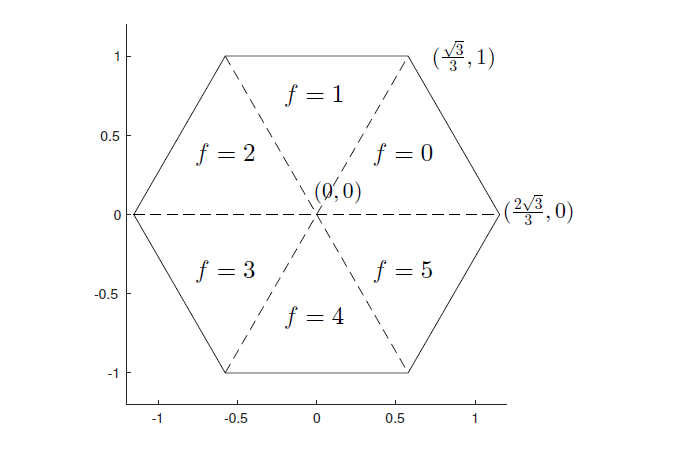
\includegraphics[width=8cm]{tu.png}
\end{figure}
\subsection{问题分析}
对于上面问题,首先边界条件为Neumman边值,但是常数c并没有给出,需要求解。通过简单分析,对于方程\eqref{eq:1},应用Gause-Green公式,得:
\begin{equation}
\begin{aligned}
\label{eq:2}
\int_{x\in\Omega} f\ dx&= \int_{x\in\Omega} -\Delta u\ dx \\
                       &=\int_{x\in\partial\Omega} -\frac{\partial u}{\partial n}\\
		       &=\int_{x\in\partial\Omega}\ -c\ dx
\end{aligned}
\end{equation}
由于$f$为分片常数,通过简单计算,得到$\int_{x\in\Omega}f\ dx=5\sqrt{3}$,而$\int_{x\in\partial\Omega}dx=4\sqrt{3}$,则$c=-\frac{5}{4}=-1.25$,这样,得到了具体的$Neumman$边值条件。\par
接下来,我们考虑网格的剖分,由于区域$\Omega$不是规则的矩阵区域,对于矩阵剖分网格来说,比较难处理,因为选择均匀的矩阵剖分,会有点落在区域外面,而且,不能保证区域的边界上,总有剖分点存在。同时,在这种情况下,点的排列也相对比较困难。\par
为了处理这种情况,同时使点的排列较为简单,我们引入虚拟节点,即对正六边形区域的四个角补上虚拟的节点,将区域补成一个标准的矩形区域,在这个矩形区域内做矩形网格剖分,就相对比较简单。\par
由于新的矩形区域,其长为:$l=\frac{4\sqrt{3}}{3}$,其宽度为:$w=2$,因此我们考虑的单位网格,长和宽不相同。假设在y方向,剖分网格数为n,则单位网格竖直方向长度$dy=\frac{2}{n}$,为了使在矩形内部与原正六边形重合部分都有单位网格点,结合图形的几何信息可知,单位网格水平方向长度满足:$\frac{dy}{dx}=\sqrt{3}$,
即$dx=\frac{dy}{\sqrt{3}}=\frac{2\sqrt{3}}{3n}$
所以,水平方向上的网格数:$m=\frac{l}{dx}=2n$。\par
最后,需要注意,为了使现在的矩形与原来正六边形端点重合的点,在剖分后的单位网格节点上,$\frac{1}{dy}=\frac{n}{2}$应该为整数,这样,n需要被2能整除。因此,综合上面的分析,我们的网格剖分,如下;
\begin{itemize}
\item 水平方向网格数:$m=4n$,竖直方向网格数:$k=2n$,$n\in N$;
\item 水平方向单位网格长度:$dx=\frac{\sqrt{3}}{3n}$,竖直方向单位网格长度:
$\frac{1}{n}$;
\item 节点总数:$m\times n=(4n+1)\times(2n+1)$,并且我们按从左到右,从下到上的顺序对节点进行标号,
即从下边界开始,第一行从左忘右:$1,2,3,\cdots,4n+1$,进行标号;上面第二行,从左往右:$4n+2,4n+3,\cdots,8n+2$,进行标号;依次类推,对于第k行,从左往右:$(4n+1)*(k-1)+1,(4n+1)*(k-1)+2,\cdots,(4n+1)*k,\ k=1,2,\cdots,2n+1$。\par
所以,任意第i行j列的节点(i,j)其标号为:$(4n+1)*(i-1)+j,1\leq i\leq 2n+1,\ 1\leq j \leq 4n+1$,简单的图形表示,如下:\par
\begin{figure}[h]
\centering
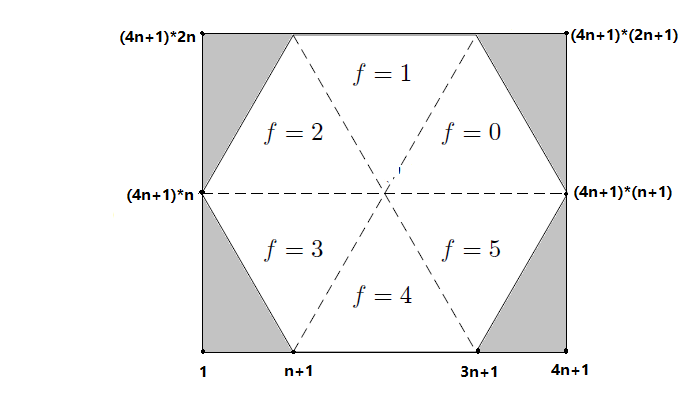
\includegraphics[width=8cm]{tu1.png}
\label{fig:1}
\end{figure}
\end{itemize}
图中,阴影部分表示引入的虚拟节点。这样,对于边值条件的计算,网格的剖分以及节点的排列已经处理完成,下面对节点进行具体的差分处理。
\section{差分格式}
\subsection{虚拟节点的处理}
我们引入虚拟节点,使节点的排序变得方便,但是这样网格节点数目却增加了。因此,在差分处理时,我们根据排序信息,较容易的确定该点是引入的虚拟节点,还是在正六边形内部的或边界上,因为我们真正关系的点的信息,是在正六边形内部或边界上。\par
例如,对与第k行,$0<=k<n$时,第$k*(4n+1)+1$个节点,到$k*(4n+1)+n-k$个节点,以及$k*(4n+1)+3n+1+k$到$(k+1)*(4n+1)$都是虚拟节点。
这样,在节点差分时,不考虑这些节点,即不对这些节点做任何操作。
\subsection{正六边形端点的处理}
由于,题目所给的边界条件是Neumman边值,对于正六边形的端点,其不具有连续性,因此会存在两种可能的边值情况,因此我们做了如下约定:
\begin{itemize}
\item 对于下边界上两端点,其外法向方向与下边界的外法向方向相同,即满足下边界边界条件;
\item 对于上边界上两端点,其外法相方向与上边界的外法向方向相同,即满足上边界边界条件;
\item 对于左端点,其外法向方向,平行x轴向左,即指向x轴反方向。其边界条件满足:$\frac{\partial u_{i,j}}{\partial n}=(u_{i,j}-u_{i,j+1})/dx=c,\ i=n,\ j=1$
\item 对于右端点,其外法向方向,平行x轴向右,即指向x轴正方向。其边界条件满足:$\frac{\partial u_{i,j}}{\partial n}=(u_{i,j}-u_{i,j-1})/dx=c,\ i=n,\ j=4n+1$。
\end{itemize}
\subsection{正六边形边界点的差分}
参考图形\ref{fig:1},我们从$f=5$区域的边界开始,逆时针方向将边界标记为:$1,2,3,4,5,6$。已知:\par
\begin{equation}
\label{eq:3}
\frac{\partial u}{\partial n}=\nabla u \cdot \vec{n}=(\frac{\partial u}{\partial x},\frac{\partial u}{\partial y})\cdot (n_1,n_2) 
\end{equation}
其中,$\nabla u$ 为u的梯度,$\vec{n}$为单位外法向。则有:\par
\begin{itemize}
\item 对于1号边界,$\vec{n}=(\frac{\sqrt{3}}{2},-\frac{1}{2})$,$\nabla u=(\frac{u_{i,j}-u_{i,j-1}}{dx},\frac{u_{i+1,j}-u_{i,j}}{dy})$,因此,由\eqref{eq:3},其边界条件满足:
\begin{equation*}
\frac{\sqrt{3}}{2}\frac{u_{i,j}-u_{i,j-1}}{dx}+\frac{1}{2}\frac{u_{i,j}-u_{i+1,j}}{dy}=c;\ 1\leq i\leq n-1,\ j=3*n+i
\end{equation*}
\item 对于2号边界,$\vec{n}=(\frac{\sqrt{3}}{2},\frac{1}{2})$,$\nabla u=(\frac{u_{i,j}-u_{i,j-1}}{dx},\frac{u_{i,j}-u_{i-1,j}}{dy})$,因此,由\eqref{eq:3},其边界条件满足:
\begin{equation*}
\frac{\sqrt{3}}{2}\frac{u_{i,j}-u_{i,j-1}}{dx}+\frac{1}{2}\frac{u_{i,j}-u_{i-1,j}}{dy}=c;\ n+1\leq i\leq 2n-1,\ j=5n-i;
\end{equation*}
\item 对于3号边界,$\vec{n}=(0,1)$,$\nabla u=(0,\frac{u_{i,j}-u_{i-1,j}}{dy})$,因此,由\eqref{eq:3},其边界条件满足:
\begin{equation*}
\frac{u_{i,j}-u_{i-1,j}}{dy}=c;\ i=2n,\ n+1\leq j\leq 3n+1;
\end{equation*}
\item 对于4号边界,$\vec{n}=(-\frac{\sqrt{3}}{2},\frac{1}{2})$,$\nabla u=(\frac{u_{i,j+1}-u_{i,j}}{dx},\frac{u_{i,j}-u_{i-1,j}}{dy})$,因此,由\eqref{eq:3},其边界条件满足:
\begin{equation*}
\frac{\sqrt{3}}{2}\frac{u_{i,j}-u_{i,j+1}}{dx}+\frac{1}{2}\frac{u_{i,j}-u_{i-1,j}}{dy}=c;\ 1+n\leq i\leq 2n-1,\ j=i-n;
\end{equation*}
\item 对于5号边界,$\vec{n}=(\frac{-\sqrt{3}}{2},-\frac{1}{2})$,$\nabla u=(\frac{u_{i,j+1}-u_{i,j}}{dx},\frac{u_{i+1,j}-u_{i,j}}{dy})$,因此,由\eqref{eq:3},其边界条件满足:
\begin{equation*}
\frac{\sqrt{3}}{2}\frac{u_{i,j}-u_{i,j+1}}{dx}+\frac{1}{2}\frac{u_{i,j}-u_{i+1,j}}{dy}=c;\ 1\leq i\leq n-1,\ j=n-i;
\end{equation*}
\item 对于6号边界,$\vec{n}=(0,-1)$,$\nabla u=(0,\frac{u_{i+1,j}-u_{i,j}}{dy})$,因此,由\eqref{eq:3},其边界条件满足:
\begin{equation*}
\frac{u_{i,j}-u_{i+1,j}}{dy}=c;\ i=0,\ n+1\leq j=\leq 3n+1
\end{equation*}
\end{itemize}
\subsection{内部节点的差分}
在上面,我们已经对原来正六边形边界上的点(包括端点)做了差分处理,现在剩下的就只有正六边形内部的节点。由于我们的网格剖分是矩形,
显然,最简单直接的办法是采用二阶中心差分,例如对i行j列的节点(i,j),其差分格式为:\par
\begin{equation}
\label{eq:4}
\Delta u_{i,j}=\frac{\partial^2 u}{\partial x^2}|_{i,j}+\frac{\partial^2 u}{\partial y^2 }|_{i,j}=\frac{u_{i,j+1}+u_{i,j-1}-2u_{i,j}}{dx^2}+\frac{u_{i+1,j}+u_{i-1,j}-2u_{i,j}}{dy^2}=f
\end{equation}
其中,(i,j)满足:\par
\begin{itemize}
\item 当$0<i<n$时,$n-i<j<3n+i$;
\item 当$i=n$时,$1<j<4n+1$;
\item 当$n<i<2n$时,$i-n<j<5n-i$;
\end{itemize}
\subsection{泊松方程右端项处理}
对于泊松方程$\Delta u=f$,由于f在正六边形内是分片常数,如图:\ref{fig:1}。我们从$f=0$开始逆时针方向,将f标记为:$f0,f1,f2,f3,f4,f5$,其中fi表示,$fi=i,i=0,1,2,3,4,5$。\par
而在处理图\ref{fig:1}中所示的虚线部分的f的值时,我们选择f相同的划分方式式,从右端水平虚线开始,逆时针方向记为:$0,1,2,3,4,5$号,其中,每个标号,代表了在其虚线上的点处,f的取值。
因此,我们有如下划分:\par
\begin{itemize}
\item 当$0<i<n$,$n-i<j<3n+i$时为内部节点,其中,若$n-i<j<n+i,\ f=f3 $,若$3n-i\leq j<3n+i,\ f=f5 $,否则$f=f4$;
\item 当$i=n$,$1<j<4n+1$时为中心水平虚线上点,其中,若$1<j\leq 2n+1,\ f=f3$,否则$f=f0$;
\item 当$n<i<2n$,$i-n<j<5n-i$时,也为内部节点,其中,若$i-n<j\leq 3n-i,\ f=f2$,若$3n-i<j\leq n+i,\ f=f1$,否则$f=f0$;
\end{itemize}
这样,对于任意内部节点(i,j),我们便可以知道,其对应的泊松方程右端项,f的取值。
\subsection{化简差分格式}
由于我们选取的矩形网格剖分,因此单位网格的长和宽满足:$\frac{dy}{dx}=\sqrt{3}$和$\frac{dy^2}{dx^2}$这样,对于上面正六边形关于边界点(包括端点)和内部
点的差分格式,我们统一的将左端式子中分母的单位网格尺寸(dy和dx)放到等式的右端项中,这样便可以得到相对简单的差分表达式:
\begin{itemize}
\item 对于左端点:$u_{i,j}-u_{i,j+1}=dx*c,\ i=n,j=1$;对于右端点:$u_{i,j}-u_{i,j-1}=dx*c,\ i=n,j=4n+1$;
\item 对于1号边界点:$4u_{i,j}-3u_{i,j-1}-u_{i+1,j}=2dy*c;\ 1\leq i\leq n-1,\ j=3*n+i$;
\item 对于2号边界点:$4u_{i,j}-3u_{i,j-1}-u_{i-1,j}=2dy*c;\ n+1\leq i\leq 2n-1,\ j=5n-i$;
\item 对于3号边界点:$u_{i,j}-u_{i-1,j}=dy*c,\ i=2n,n+1\leq j\leq 3n+1$;
\item 对于4号边界点:$4u_{i,j}-3u_{i,j+1}-u_{i-1,j}=2dy*c,\ n+1\leq i\leq 2n-1,\ j=i-n$;
\item 对于5号边界点:$4u_{i,j}-3u_{i,j+1-u_{i+1,j}}=2dy*c,\ 1\leq i\leq n-1,\ j=n-i$;
\item 对于6号边界点:$u_{i,j}-u_{i+1,j}=dy*c,\ i=0,\ n+1\leq j\leq 3n+1$;
\item 对于内部节点: $8u_{i,j}-3u_{i,j-1}-3u_{i,j+1}-u_{i-1,j}-u_{i+1,j}=dy^2*f $,
其中,当$0<i<n$时,$n-i<j<3n+i$;当$i=n$时,$1<j<4n+1$,当$n<i<2n$时,$i-n<j<5n-i$。而关于f的取值,在上面右端项的处理中,已经明确的给出。
\end{itemize}
\section{系数矩阵和右端项的存储}
在上面,我们已经给出了具体的差分格式,即对于任意(i,j)点,能很容易也清楚的知道其满足的差分方程。因此,综合上面的信息,我们便可以将带Neumman边值
条件的泊松方程,通过差分近似的方式,将求解原方程转化为求解线性方程组:$A0*x=b$。其中,A0对应通过差分格式得到的系数矩阵,x对应为未知的u,b对应为右端项f。\par
由于网格剖分一共有$m*n$个节点,则对应的系数矩阵A0应该有$m*n$行和$m*n$列,x和b也为$m*n$的列向量。其中,x和b的第i行,表示第i个节点的值和对应的右端项f的值。因此,相应的A的第i行
表示第i个节点的差分方程的系数。$1\leq i<\leq m*n$ \par
观察上面的差分方程,可以发现,对于系数矩阵A0的每一行,最多只有5个非0元素。这样,为了节省内存,我们将系数采取稀疏存储的方式,用矩阵A表示,其中A为$m*n$行,5列的矩阵。需要注意的是,对于A的任意第i行,当i属于内部节点时:\par
\begin{itemize}
\item 矩阵A的第一列,A(i,1)对应于第i个节点前第i-m个节点的系数;
\item 矩阵A的第二列,A(i,2)对应于第i个节点前第i-1个节点的系数;
\item 矩阵A的第三列,A(i,3)对应于第i个节点本身的系数;
\item 矩阵A的第四列,A(i,4)对应于第i个节点后第i+1个节点的系数;
\item 矩阵A的第五列,A(i,5)对应于第i个节点后第i+m个节点的系数;
\end{itemize}
即我们将矩阵A任意第i行每列的系数,与第i个节点周围空间位置的信息相联系,每一列都对应于第i个节点周围节点的空间位置。这样,在处理矩阵乘向量时,遵从通常矩阵乘向量的规则,即对应位置对应相乘即可,例如:原来线性方程组A0*x=b的第i行,等价于\par
\begin{equation*}
A_{i,1}*x_{i-m}+A_{i,2}*x_{i-1}+A_{i,3}*x_{i}+A_{i,4}*x_{i+1}+A_{i,5}*x_{i+m}=b_i
\end{equation*}
而当i不是内部节点时,存在两种情况,i节点在正六边形边界上,此时矩阵A0第i行的非0系数,小于5,本质上也满足上面的对应关系,但需要特别注意和处理。例如:
当对于第i个节点,若$i-m$,$i-1$,$i+1$,$i+m$任意之一对应的节点位置,在正六边形之外时,我们令矩阵A第i行相对应的列系数为0。这样,在处理矩阵A乘向量x时,也满足上面的对应式:\par
\begin{equation*}
A_{i,1}*x_{i-m}+A_{i,2}*x_{i-1}+A_{i,3}*x_{i}+A_{i,4}*x_{i+1}+A_{i,5}*x_{i+m}=b_i
\end{equation*}
而若(i-m)节点不在正六边形内,相应项:$A(i,1)*x(i-m)=0$,即在第i行的方程中不存在该项。
综上所述,采取稀疏存储以及矩阵A任意i行j列,与第i个节点,周围节点空间位置相对应的关系,使的存储空间减小,且保留了原来的矩阵A0有用的信息。因为,原来线性方程组
$A0*x=b$的第i行,等于现在A的第i行与x对应位置相乘。
而当第i节点不在正六边形内部时,相应的矩阵A0的第i行系数全部为0,此时我们也设A的第i行系数为0,这样在处理矩阵A与x对应位置相乘时,引入的虚拟节点并没有实际参与计算。\par

将上面所述的格式整理成矩阵形式,矩阵如下:\par

\[
\left[\begin{array}{cccccc}
  a_{1,1} &a_{1,2} &a_{1,3} &a_{1,4} &a_{1,5}\\
   \vdots &\vdots &\vdots &\vdots &\vdots  \\
  a_{i,1} &a_{i,2} &a_{i,3} &a_{i,4} &a_{i,5}\\
  a_{i+1,1} &a_{i+1,2} &a_{i+1,3} &a_{i+1,4} &a_{i+1,5}\\
  a_{i+2,1} &a_{i+2,2} &a_{i+2,3} &a_{i+2,4} &a_{i+2,5}\\
   \vdots &\vdots &\vdots &\vdots &\vdots  \\
  a_{m*n,1} &a_{m*n,2} &a_{m*n,3} &a_{m*n,4} &a_{m*n,5}
\end{array}\right]x=\left[\begin{array}{c}
  b_1\\
  b_2\\
  b_3\\
  \vdots\\
  b_{m*n-1}\\
  b_{m*n}
\end{array}\right]\]

其中,对于任意i节点:\par
\begin{itemize}
\item 若不在正六边形上,则$a_{i,1}=a_{i,2}=a_{i,3}=a_{i,4}=a_{i,5}=0$,
\item 若其为正六边形左端点,$a_{i,3}=1,a_{i,4}=-1$,若为右端点,$a_{i,3}=1,a_{i,2}=-1$,矩阵第i行其余值为0,
\item 若其在正六边形下边界上,$a_{i,3}=1,a_{i,5}=-1$,矩阵第i行其余的值为0,
\item 若其在正六边形上边界上,$a_{i,3}=1,a_{i,1}=-1$,矩阵第i行其余值为0,
\item 若其在正六边形左下边界上,$a_{i,3}=4,a_{i,4}=-3,a_{i,5}=-1$,矩阵第i行其余的值为0,
\item 若其在正六边形左上边界上,$a_{i,3}=4,a_{i,4}=-3,a_{i,1}=-1$,矩阵第i行其余值为0,
\item 若其在正六边形右下边界上,$a_{i,3}=4,a_{i,2}=-3,a_{i,5}=-1$,矩阵第i行其余的值为0,
\item 若其在正六边形右上边界上,$a_{i,3}=4,a_{i,2}=-3,a_{i,1}=-1$,矩阵第i行其余值为0,
\item 若第i节点在正六边形内部,相应的$a_{i,1}=-1,a_{i,2}=-3,a_{i,3}=8,a_{i,4}=-3,a_{i,5}=-1$
\end{itemize}
\section{并行处理}
在并行求解线性方程组$Ax=b$时,我们先观察上面的矩阵A的系数,发现对于矩阵A,其任意第i行,行和为0。
这样,取一个$m*n$维列向量e,$e=(1,1,\cdots,1,1)^T$,可以得到,$A*e=0*e$。
则说明,$\lambda=0$为矩阵A的一个特征值,对应特征向量为e,说明矩阵A是奇异的,因此解不唯一。其实,直接分析原方程\eqref{eq:1}也可以知道,假设u为方程\eqref{eq:1}的解,则$u+C$也是该方程的解,其中C为任意常数。由定理也可知,Neumman边值的泊松方程,解不唯一。\par
因此,在使用迭代法求解时,为了能保证原来解的性质,同时又避免解不唯一,我们修改了矩阵A任意i行对角元的值,当i在正六边形区域内时,使i行为严格对角占优的,这样系数矩阵A不存在0特征值的情况,即矩阵A非奇异。\par
我们选择经典的Jacobi迭代法求解线性方程组,Jacobi迭代主要思想为,对于任意第k步迭代,$k\geq 0$,有如下关系:\par
$$x^{k+1}=-D^{-1}(L+U)x^k+D^{-1}b$$
其中,$x_k$为第k次迭代的值,$D$为$A$的对角元组成的对角阵,$L$为$A$的严格下三角矩阵,$U$为$A$的严格上三角矩阵,即$A=D+L+U$。则对于第k次迭代的任意i行,有如下关系:\par
当节点i不在正六边形区域内时,$x^{k+1}_i=x^k_i=0$,$k\geq 0$;\par
当节点i在正六边形区域内部时,
$$x^{k+1}_i=(-(A_{i,1}*x^k_{i-m}+A_{i,2}*x^k_{i-1}+A_{i,4}*x^k_{i+1}+A_{i,5}*x^k_{i+m})+b_i)/A_{i,3}$$

$\bullet$ 因此,我们的并行思想是:\par
\begin{itemize}
\item[*] 假设我们的进程数为size,则将x等分给每个进程去求解,即每次迭代中一个进程需要求解的x数量为:$m*n/k$;
\item[*] 对于任意第i号进程,$0\leq i\leq size-1$,其初始位置和终止位置定义为:\par
$begin(i)=m*n*i/size,end(i)=m*n*(i+1)/size$,初始位置为begin(i),而终止位置为end(i)-1;
\item[*] 因此在信息传递时,由Jacobi迭代关系可知,满足如下:\par
\begin{scriptsize}
\begin{lstlisting}
if (i > 0)
MPI_Send(&U[begin[i]], m, MPI_DOUBLE, i - 1, 0, MPI_COMM_WORLD);
if (rank < size - 1)
MPI_Send(&U[end[i] -m ], m, MPI_DOUBLE, i + 1, 0, MPI_COMM_WORLD);
if (i < size - 1)
MPI_Recv(&U[begin[i+1]], m, MPI_DOUBLE, i + 1, 0, MPI_COMM_WORLD, MPI_STATUS_IGNORE);    
if (i > 0)
MPI_Recv(&U[end[i-1] - m], m, MPI_DOUBLE, i - 1, 0, MPI_COMM_WORLD, MPI_STATUS_IGNORE);  
\end{lstlisting}
\end{scriptsize}
即对于第i号进程,若$0 \leq i\leq size$,则i号进程向i-1号进程传从x(begin(i))到x(begin(i)+m-1)的值;向i+1号进程传,从x(end(i)-m)到x(end(i)-1)的值;
同时,接收i-1号进程传来的从x(end(i-1)-m)到x(end(i-1)-1)的值,以及i+1号进程传来的从x(begin(i+1))到x(begin(i+1)+m-1)的值。\par
这样,在每次迭代后,进行一次信息传递,能保证任意第i号进程,能获得其进行下一次迭代所需要的所有值。
\item[*] 每个进程独立计算迭代一次的误差,我们的误差定义为前后两步x的差的二范数。即对于第i号进程,其误差计算为:
\begin{equation*}
error(i)=\sqrt{\sum_{j=begin(i)}^{j=end(i)-1}(x^{k+1}(j)-x^k(j))^2}
\end{equation*}
然后将其传送给0号进程,由0号进程负责计算前后两次迭代,总的误差:\par
\begin{equation*}
Error=\sum_{i=0}^{size-1}error(i)
\end{equation*}
之后将总的误差Error,广播给所有进程,由每个进程独立判断,迭代是否终止。
\item[*] 判断迭代终止的条件为:$Error<eps$且$k<Nmax$,其中eps为误差精度,Nmax为最大迭代次数。
\item[*] 当迭代终止后,第i个进程,$i\neq 0$将x(begin(i))到x(end(i)-1)传送给0号进程,由0号进程负责接收其他进程传递的x的部分信息,构成完整的解x。如下:\par
\begin{scriptsize}
\begin{lstlisting}
if(i!=0)
MPI_Send(&U[begin[i]], end[i] - begin[i], MPI_DOUBLE,0,0,MPI_COMM_WORLD);  
if(i==0)
for(int i = 1; i < size; i++)
MPI_Recv(&U[begin[i]], end[i] - begin[i], MPI_DOUBLE, i,0, MPI_COMM_WORLD, MPI_STATUS_IGNORE);   
\end{lstlisting}
\end{scriptsize}
\end{itemize}
\section{数值结果}
我们取$k=100$时的情况,此时,横向网格数$m=401$,纵向网格数$n=201$,最大迭代次数为:$Kmax=10^4$时;\par
\begin{table}[h]
\centering
\begin{tabular}{|c|c|c|c|c|}
\hline
进程数 &误差 &时间 &相对加速比 &效率  \\
\hline
1 &2.10784e-5  &9.91s   &1   &1  \\
\hline
2 &2.10784e-51 &5.25s   &1.8876  & 0.9438   \\
\hline
3 &2.10784e-5  &4.22s  &2.3483   &0.7827 \\
\hline
4 &2.10784-e   &3.47s   &2.8724   & 0.7181     \\
\hline
5 &2.10784e-5   &3.99s   &2.4837   &0.4967   \\
\hline
8 &2.10784e-5   &6.28s    &1.5780  &0.1972  \\
\hline
\end{tabular}
\end{table}
\newpage
从中可以看出,当进程数小于4的时候,相对于一个进程的加速比基本在2以上,且并行效率也保持在0.7以上,处于相对合理的范围内。但是,当进程数大于5之后,并行效率就大大降低,这是因为我用于计算的电脑最多只有4个核,当满核操作的时候,效率会大大降低,一般保证效率时,只需要用到电脑$\frac{1}{2}$的核数。\par
\par
下面将画出$N=100$和$N=50$时的计算结果图,此时的误差为:$Error=1.5395e-5$ \par
\par
\begin{figure}[ht]
\label{fig:3}
\centering 
\subfigure[$N=50$时的计算结果]{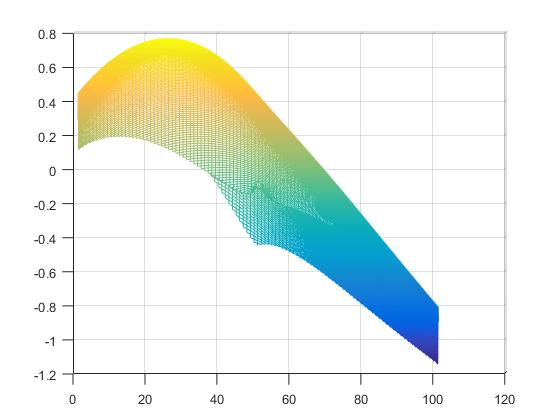
\includegraphics[scale=0.4]{result3.jpg}}
\subfigure[$N=100$时的计算结果]{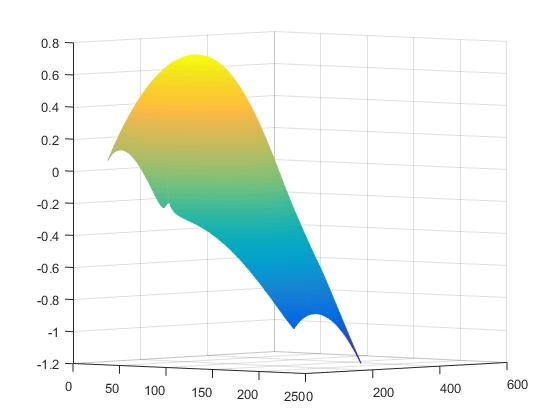
\includegraphics[scale=0.4]{result2.jpg}}
\end{figure}
从上图\ref{fig:3}可以看出,这两幅图形状相似,只是从不同的角度观察的。发现当网格加密时,得到的结果更光滑,但是这样会增大计算量。以上两幅图都是4个进程时,取不同的网格数得到的结果。当取其他进程数时,得到的结果与上面结果相似,就不再一一列举了。
\end{document} 
